% Options for packages loaded elsewhere
\PassOptionsToPackage{unicode}{hyperref}
\PassOptionsToPackage{hyphens}{url}
\PassOptionsToPackage{dvipsnames,svgnames,x11names}{xcolor}
%
\documentclass[
  letterpaper,
  DIV=11,
  numbers=noendperiod,
  oneside]{scrartcl}

\usepackage{amsmath,amssymb}
\usepackage{iftex}
\ifPDFTeX
  \usepackage[T1]{fontenc}
  \usepackage[utf8]{inputenc}
  \usepackage{textcomp} % provide euro and other symbols
\else % if luatex or xetex
  \usepackage{unicode-math}
  \defaultfontfeatures{Scale=MatchLowercase}
  \defaultfontfeatures[\rmfamily]{Ligatures=TeX,Scale=1}
\fi
\usepackage{lmodern}
\ifPDFTeX\else  
    % xetex/luatex font selection
\fi
% Use upquote if available, for straight quotes in verbatim environments
\IfFileExists{upquote.sty}{\usepackage{upquote}}{}
\IfFileExists{microtype.sty}{% use microtype if available
  \usepackage[]{microtype}
  \UseMicrotypeSet[protrusion]{basicmath} % disable protrusion for tt fonts
}{}
\makeatletter
\@ifundefined{KOMAClassName}{% if non-KOMA class
  \IfFileExists{parskip.sty}{%
    \usepackage{parskip}
  }{% else
    \setlength{\parindent}{0pt}
    \setlength{\parskip}{6pt plus 2pt minus 1pt}}
}{% if KOMA class
  \KOMAoptions{parskip=half}}
\makeatother
\usepackage{xcolor}
\usepackage[left=1in,marginparwidth=2.0666666666667in,textwidth=4.1333333333333in,marginparsep=0.3in]{geometry}
\setlength{\emergencystretch}{3em} % prevent overfull lines
\setcounter{secnumdepth}{-\maxdimen} % remove section numbering
% Make \paragraph and \subparagraph free-standing
\ifx\paragraph\undefined\else
  \let\oldparagraph\paragraph
  \renewcommand{\paragraph}[1]{\oldparagraph{#1}\mbox{}}
\fi
\ifx\subparagraph\undefined\else
  \let\oldsubparagraph\subparagraph
  \renewcommand{\subparagraph}[1]{\oldsubparagraph{#1}\mbox{}}
\fi


\providecommand{\tightlist}{%
  \setlength{\itemsep}{0pt}\setlength{\parskip}{0pt}}\usepackage{longtable,booktabs,array}
\usepackage{calc} % for calculating minipage widths
% Correct order of tables after \paragraph or \subparagraph
\usepackage{etoolbox}
\makeatletter
\patchcmd\longtable{\par}{\if@noskipsec\mbox{}\fi\par}{}{}
\makeatother
% Allow footnotes in longtable head/foot
\IfFileExists{footnotehyper.sty}{\usepackage{footnotehyper}}{\usepackage{footnote}}
\makesavenoteenv{longtable}
\usepackage{graphicx}
\makeatletter
\def\maxwidth{\ifdim\Gin@nat@width>\linewidth\linewidth\else\Gin@nat@width\fi}
\def\maxheight{\ifdim\Gin@nat@height>\textheight\textheight\else\Gin@nat@height\fi}
\makeatother
% Scale images if necessary, so that they will not overflow the page
% margins by default, and it is still possible to overwrite the defaults
% using explicit options in \includegraphics[width, height, ...]{}
\setkeys{Gin}{width=\maxwidth,height=\maxheight,keepaspectratio}
% Set default figure placement to htbp
\makeatletter
\def\fps@figure{htbp}
\makeatother
\newlength{\cslhangindent}
\setlength{\cslhangindent}{1.5em}
\newlength{\csllabelwidth}
\setlength{\csllabelwidth}{3em}
\newlength{\cslentryspacingunit} % times entry-spacing
\setlength{\cslentryspacingunit}{\parskip}
\newenvironment{CSLReferences}[2] % #1 hanging-ident, #2 entry spacing
 {% don't indent paragraphs
  \setlength{\parindent}{0pt}
  % turn on hanging indent if param 1 is 1
  \ifodd #1
  \let\oldpar\par
  \def\par{\hangindent=\cslhangindent\oldpar}
  \fi
  % set entry spacing
  \setlength{\parskip}{#2\cslentryspacingunit}
 }%
 {}
\usepackage{calc}
\newcommand{\CSLBlock}[1]{#1\hfill\break}
\newcommand{\CSLLeftMargin}[1]{\parbox[t]{\csllabelwidth}{#1}}
\newcommand{\CSLRightInline}[1]{\parbox[t]{\linewidth - \csllabelwidth}{#1}\break}
\newcommand{\CSLIndent}[1]{\hspace{\cslhangindent}#1}

\usepackage{fontawesome5}
\KOMAoption{captions}{tableheading}
\makeatletter
\makeatother
\makeatletter
\makeatother
\makeatletter
\@ifpackageloaded{caption}{}{\usepackage{caption}}
\AtBeginDocument{%
\ifdefined\contentsname
  \renewcommand*\contentsname{Table of contents}
\else
  \newcommand\contentsname{Table of contents}
\fi
\ifdefined\listfigurename
  \renewcommand*\listfigurename{List of Figures}
\else
  \newcommand\listfigurename{List of Figures}
\fi
\ifdefined\listtablename
  \renewcommand*\listtablename{List of Tables}
\else
  \newcommand\listtablename{List of Tables}
\fi
\ifdefined\figurename
  \renewcommand*\figurename{Figure}
\else
  \newcommand\figurename{Figure}
\fi
\ifdefined\tablename
  \renewcommand*\tablename{Table}
\else
  \newcommand\tablename{Table}
\fi
}
\@ifpackageloaded{float}{}{\usepackage{float}}
\floatstyle{ruled}
\@ifundefined{c@chapter}{\newfloat{codelisting}{h}{lop}}{\newfloat{codelisting}{h}{lop}[chapter]}
\floatname{codelisting}{Listing}
\newcommand*\listoflistings{\listof{codelisting}{List of Listings}}
\makeatother
\makeatletter
\@ifpackageloaded{caption}{}{\usepackage{caption}}
\@ifpackageloaded{subcaption}{}{\usepackage{subcaption}}
\makeatother
\makeatletter
\@ifpackageloaded{tcolorbox}{}{\usepackage[skins,breakable]{tcolorbox}}
\makeatother
\makeatletter
\@ifundefined{shadecolor}{\definecolor{shadecolor}{rgb}{.97, .97, .97}}
\makeatother
\makeatletter
\makeatother
\makeatletter
\@ifpackageloaded{sidenotes}{}{\usepackage{sidenotes}}
\@ifpackageloaded{marginnote}{}{\usepackage{marginnote}}
\makeatother
\makeatletter
\makeatother
\ifLuaTeX
  \usepackage{selnolig}  % disable illegal ligatures
\fi
\IfFileExists{bookmark.sty}{\usepackage{bookmark}}{\usepackage{hyperref}}
\IfFileExists{xurl.sty}{\usepackage{xurl}}{} % add URL line breaks if available
\urlstyle{same} % disable monospaced font for URLs
\hypersetup{
  pdftitle={Hanne Oberman},
  colorlinks=true,
  linkcolor={blue},
  filecolor={Maroon},
  citecolor={Blue},
  urlcolor={Blue},
  pdfcreator={LaTeX via pandoc}}

\title{Hanne Oberman}
\usepackage{etoolbox}
\makeatletter
\providecommand{\subtitle}[1]{% add subtitle to \maketitle
  \apptocmd{\@title}{\par {\large #1 \par}}{}{}
}
\makeatother
\subtitle{Statistician, interdisciplinarian, open scientist}
\author{}
\date{}

\begin{document}
\maketitle
\begin{center}
\href{mailto:h.i.oberman@uu.nl}{\faIcon{envelope}}
\href{http://hanneoberman.github.io}{\faIcon{github}}
\href{https://orcid.org/0000-0003-3276-2141}{\faIcon{orcid}}
\href{http://github.com/hanneoberman}{\faIcon{github}}
\href{https://www.linkedin.com/in/hanneoberman}{\faIcon{linkedin}}
\href{https://mastodon.social/@oberman}{\faIcon{mastodon}}
\href{https://twitter.com/hioberman}{\faIcon{twitter}}
\end{center}
% <a href=mailto:h.i.oberman@uu.nl class="fa fa-envelope"></a>
% <a href=http://hanneoberman.github.io/ class="fa fa-home"></a>
% <a href=https://orcid.org/0000-0003-3276-2141 class="ai ai-orcid"></a>
% <a href=http://github.com/hanneoberman/ class="fa-brands fa-github"></a>
% <a href=https://www.linkedin.com/in/hanneoberman/ class="fa-brands fa-linkedin"></a>
% <a href=https://mastodon.social/@oberman class="fa-brands fa-mastodon"></a>
% <a href=https://twitter.com/hioberman class="fa-brands fa-twitter"></a>

\ifdefined\Shaded\renewenvironment{Shaded}{\begin{tcolorbox}[breakable, boxrule=0pt, interior hidden, enhanced, borderline west={3pt}{0pt}{shadecolor}, sharp corners, frame hidden]}{\end{tcolorbox}}\fi

\begin{center}\rule{0.5\linewidth}{0.5pt}\end{center}

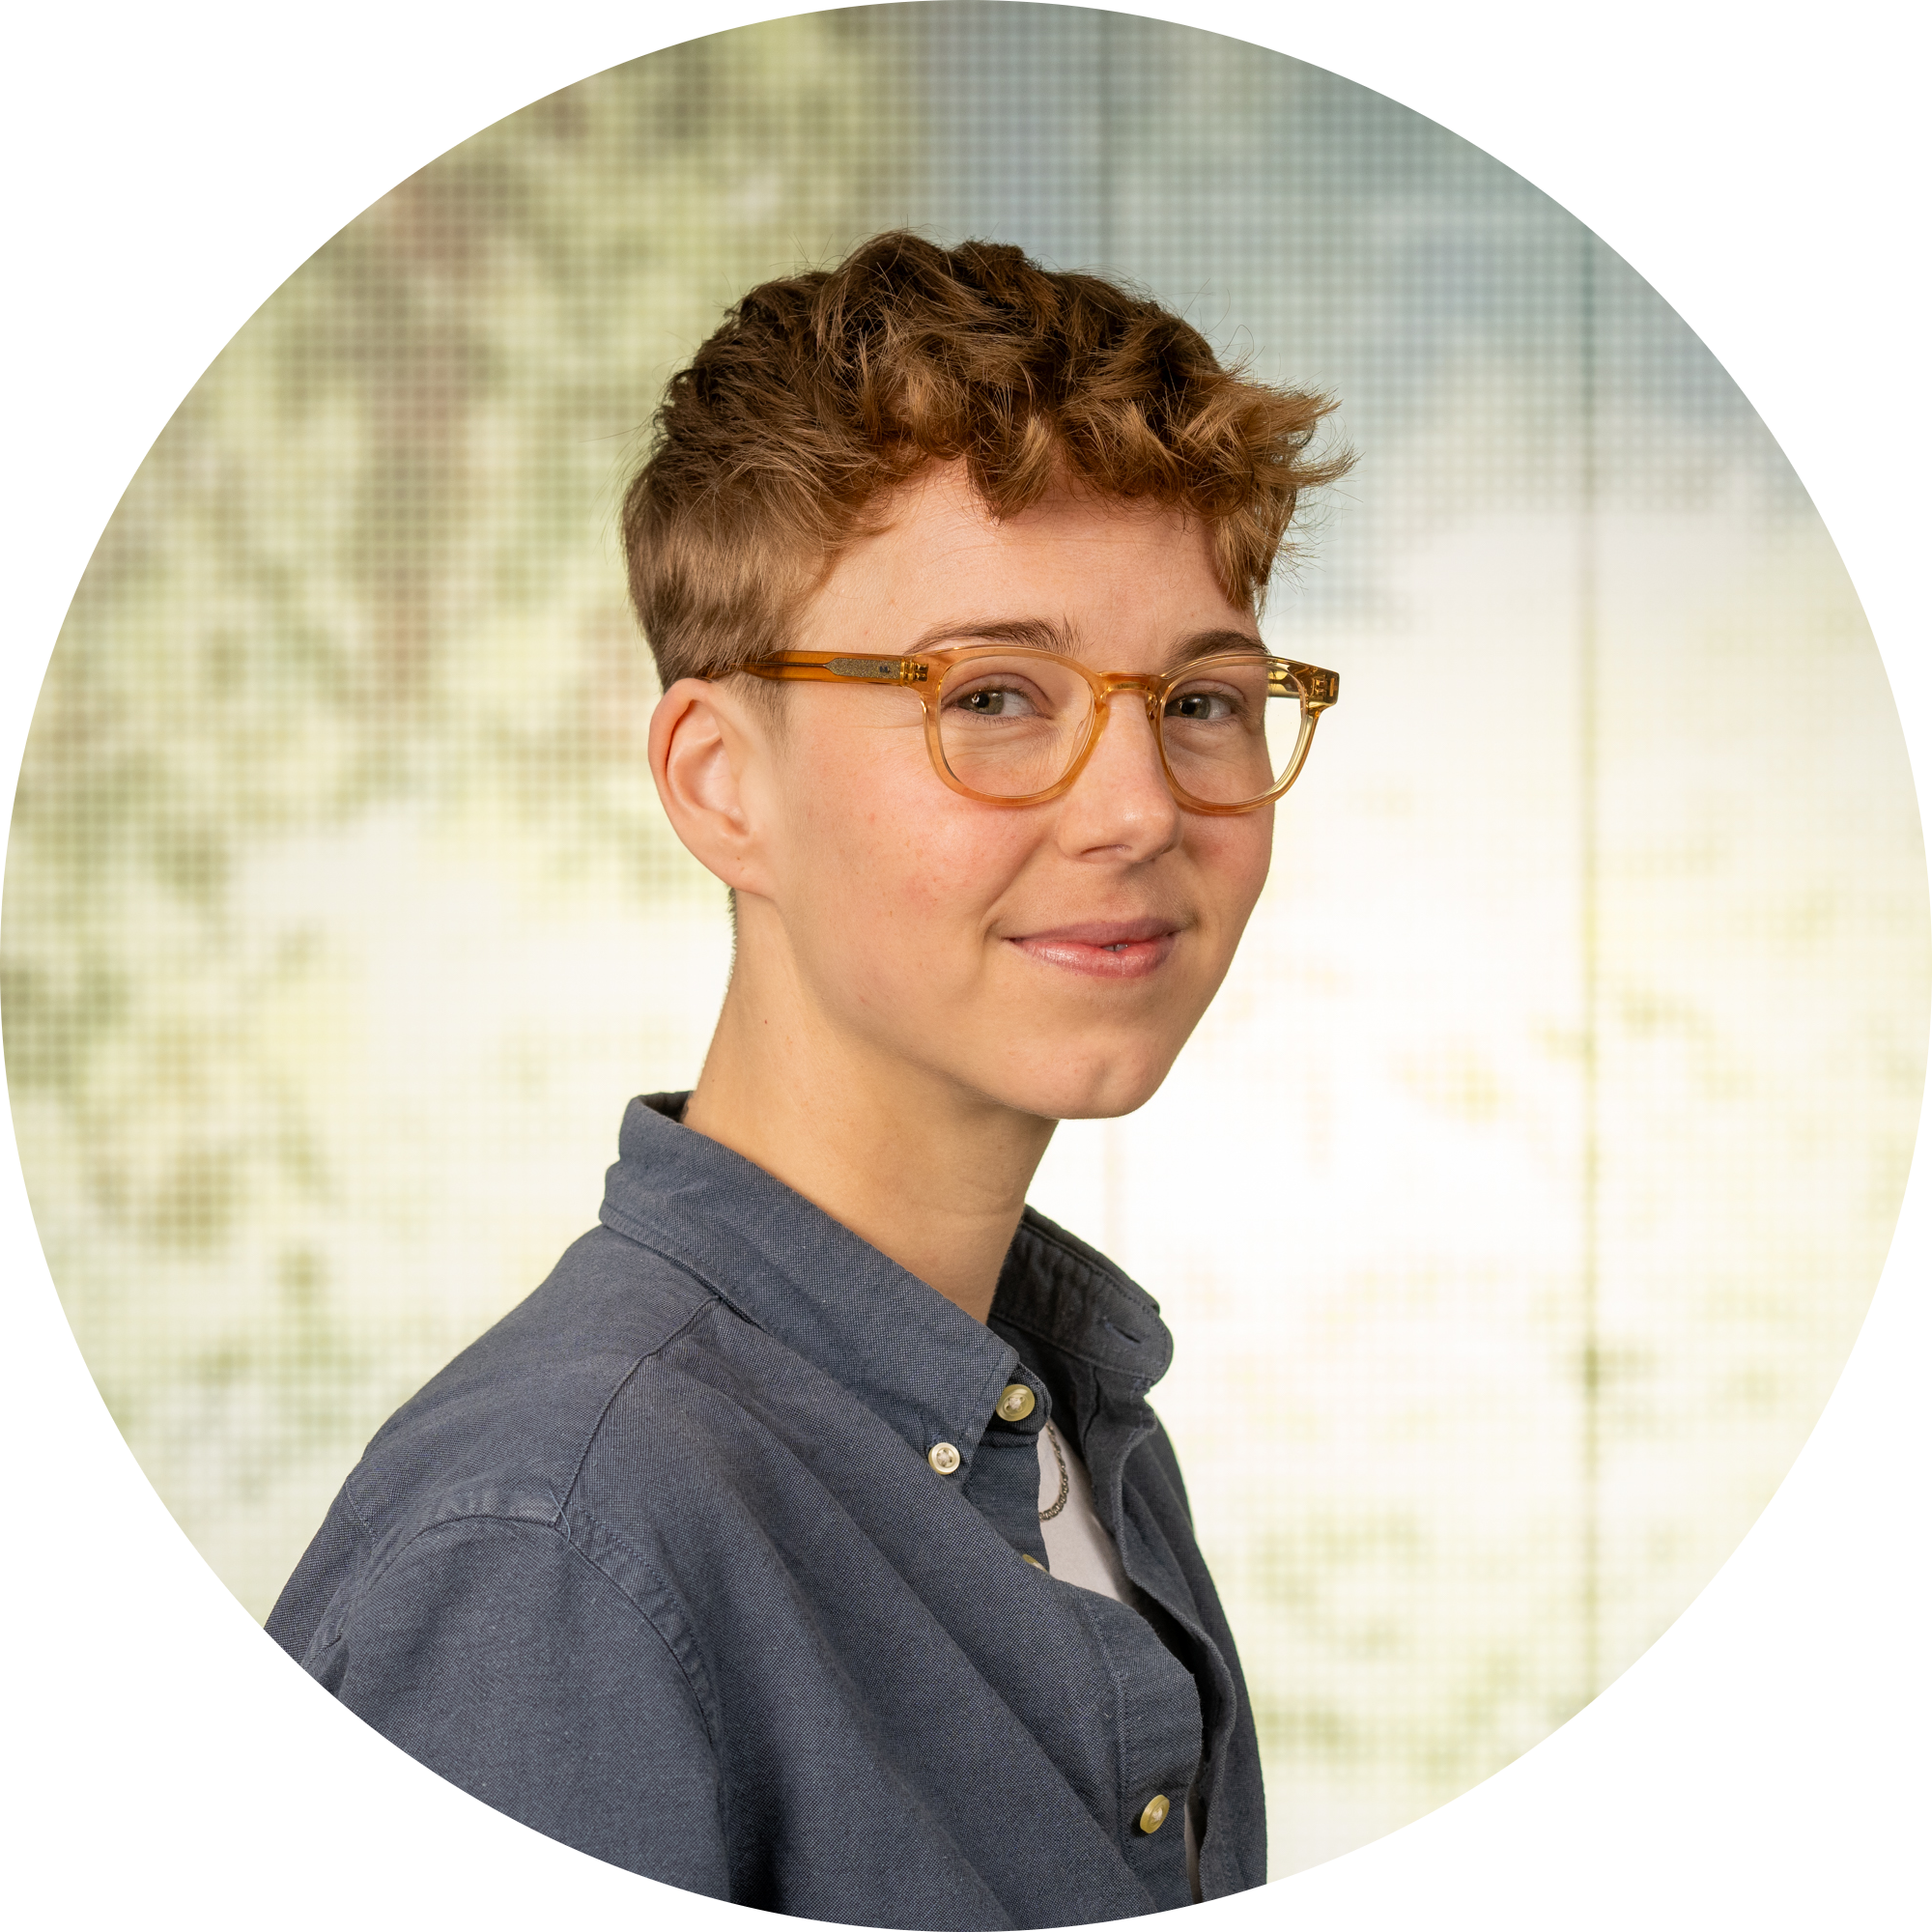
\includegraphics{avatar.png}

I am very passionate about `dull' or `difficult' topics such as
statistics, programming, and philosophy of science. I'm motivated to use
my enthusiasm and expertise to improve the quality of academic research
and education. I aspire to (help others to) solve complex real-world
problems that require insights from many disciplines and methodologies.

\hypertarget{experience}{%
\subsection{Experience}\label{experience}}

{\marginnote{\begin{footnotesize}2023-current\end{footnotesize}}}

\begin{itemize}
\tightlist
\item
  PhD candidate
  \href{https://www.uu.nl/en/organisation/methodology-and-statistics}{Methodology
  and Statistics} \textbar{} Utrecht University \textbar{} Utrecht, The
  Netherlands
\end{itemize}

{\marginnote{\begin{footnotesize}2022-current\end{footnotesize}}}

\begin{itemize}
\tightlist
\item
  Faculty ambassador \href{https://openscience-utrecht.com/}{Open
  Science Community Utrecht} \textbar{} Utrecht University \textbar{}
  Utrecht, The Netherlands
\end{itemize}

{\marginnote{\begin{footnotesize}2020-2022\end{footnotesize}}}

\begin{itemize}
\tightlist
\item
  Research and education officer
  \href{https://www.uu.nl/en/organisation/methodology-and-statistics}{Methodology
  and Statistics} and
  \href{https://juliuscentrum.umcutrecht.nl/en/}{Julius Center for
  Health Sciences and Primary Care} \textbar{} Utrecht University
  \textbar{} Utrecht, The Netherlands
\end{itemize}

\hypertarget{education}{%
\subsection{Education}\label{education}}

{\marginnote{\begin{footnotesize}2023-current\end{footnotesize}}}

\begin{itemize}
\tightlist
\item
  Graduate school, Interuniversity Graduate School of Psychometrics and
  Sociometrics (IOPS), an institute for the advanced dissertation
  training in psychometrics and sociometrics of PhD students in the
  Netherlands and Belgium.
\end{itemize}

{\marginnote{\begin{footnotesize}2018-2020\end{footnotesize}}}

\begin{itemize}
\tightlist
\item
  MSc
  \href{https://www.uu.nl/en/masters/methodology-and-statistics-behavioural-biomedical-and-social-sciences}{Methodology
  and Statistics for the Behavioural, Biomedical and Social Sciences}
  \textbar{} Utrecht University \textbar{} Utrecht, The Netherlands
\end{itemize}

{\marginnote{\begin{footnotesize}2018\end{footnotesize}}}

\begin{itemize}
\item
  Post-graduate education
  \href{https://www.concordia.ca/summer/artsci/Previous-Summer-Schools/2018/GALA2018.html}{International
  Graduate Summer School of the Global Academy of Liberal Arts}
  \textbar{} Concordia University, Montreal, Canada
\end{itemize}

{\marginnote{\begin{footnotesize}2016-2018\end{footnotesize}}}

\begin{itemize}
\item
  Honours degree
  \href{https://students.uu.nl/en/academics/honours/programmes/descartes-college}{Descartes
  College} \textbar{} Utrecht University \textbar{} Utrecht, The
  Netherlands
\end{itemize}

{\marginnote{\begin{footnotesize}2014-2018\end{footnotesize}}}

\begin{itemize}
\tightlist
\item
  BSc
  \href{https://www.uu.nl/bachelors/liberal-arts-and-sciences}{Liberal
  Arts and Sciences} \textbar{} Utrecht University \textbar{} Utrecht,
  The Netherlands
\end{itemize}

\hypertarget{ancillary-positions}{%
\subsection{Ancillary positions}\label{ancillary-positions}}

{\marginnote{\begin{footnotesize}2021, 2023\end{footnotesize}}}

\begin{itemize}
\tightlist
\item
  Programme accreditation panel student member, in assessment cluster
  research masters social and behavioural sciences, Nederlands-Vlaamse
  Accreditatieorganisatie (NVAO)
\end{itemize}

{\marginnote{\begin{footnotesize}2019-current\end{footnotesize}}}

\begin{itemize}
\tightlist
\item
  Board, Founder and treasurer of the Methodology And Statistics Alumni
  Society (MASAS). Tasks include planning events and developing the
  network., MASAS,
\end{itemize}

{\marginnote{\begin{footnotesize}2019-2020\end{footnotesize}}}

\begin{itemize}
\tightlist
\item
  Research assistant Developing novel methods to improve the validity of
  social scientific prediction. With Dr.~Dong Nguyen and Dr.~Daniel
  Oberski. My task was to develop a reproducible pipeline for natural
  language processing with \texttt{R} and \texttt{Python}. I mostly
  focused on the prerequisites for `pre-registration' of these kinds of
  analyses.
\end{itemize}

{\marginnote{\begin{footnotesize}2017-2020\end{footnotesize}}}

\begin{itemize}
\tightlist
\item
  Teaching assistant, Teaching Methodology and Statistics and
  Experimental Psychology courses at all undergraduate levels. Tasks
  varied from practical supervision to lecturing, and from leading
  workgroups to grading assignments., Utrecht University,
\end{itemize}

{\marginnote{\begin{footnotesize}2017-2022\end{footnotesize}}}

\begin{itemize}
\tightlist
\item
  Representative advisory bodies. E.g., Think tank, Providing feedback
  and advice to the management teams of the Faculty of Social and
  Behavioural Sciences, student council Faculty of Social and
  Behavioural Sciences research masters, Programme advisory committee
  MSBBSS, president of the student council Liberal Arts and Sciences
\end{itemize}

{\marginnote{\begin{footnotesize}2014-2018\end{footnotesize}}}

\begin{itemize}
\tightlist
\item
  Board and committees, I have been an active member of the study
  association Liberal Arts and Sciences, USLAS Atlas. Positions include
  vice-president of the association, president of the parents' day
  committee, secretary of the travel committee, and student-mentorship.,
  USLAS Atlas,
\end{itemize}

{\marginnote{\begin{footnotesize}2012-2017\end{footnotesize}}}

\begin{itemize}
\tightlist
\item
  Extracurriculair sidelines: Hospitality, food sector, and
  volunteering. As a student, I have always worked part-time in
  restaurants and at a sustainable food start-up. Next to that, I have
  volunteered at an animal shelter and several cultural festivals. Tasks
  include supervision of a team of 5-10 colleagues, customer service,
  and account management., E.g., Dudok Rotterdam,
\end{itemize}

\hypertarget{grant-and-awards}{%
\subsection{Grant and awards}\label{grant-and-awards}}

{\marginnote{\begin{footnotesize}2021\end{footnotesize}}}

\begin{itemize}
\tightlist
\item
  Open Science Fund, This project aims to make the MICE functionality
  available through a restful API to accommodate a wider user group.
\end{itemize}

{\marginnote{\begin{footnotesize}2022\end{footnotesize}}}

\begin{itemize}
\tightlist
\item
  Open Science Fund, The dessert package allows you to automatically
  generate methodological appendices for your research workflows.
  https://www.gerkovink.com/dessert
\end{itemize}

{\marginnote{\begin{footnotesize}2019\end{footnotesize}}}

\begin{itemize}
\tightlist
\item
  Best poster, Social and Behavioural Sciences Graduate Poster Fair.
  Poster presentation about scientific practices around non-significant
  results: `Will You Publish Null Papers?', in collaboration with Jerry
  Wenzel., Utrecht University,
\end{itemize}

{\marginnote{\begin{footnotesize}2018\end{footnotesize}}}

\begin{itemize}
\tightlist
\item
  Fellowship award, Global Academy of Liberal Arts Annual Conference
  `Creativity and the Liberal Arts' (HUMA 887)., Concordia University,
  Montreal,
\end{itemize}

\hypertarget{conferences}{%
\subsection{Conferences}\label{conferences}}

{\marginnote{\begin{footnotesize}2023\end{footnotesize}}}

\begin{itemize}
\tightlist
\item
  Paper presentation, European Congress of Methodology, 'Towards a
  standardized evaluation of imputation methodology: potential pitfalls
  in simulation studies and a proposed course of action, EAM 2023,
  Ghent, Belgium
\end{itemize}

{\marginnote{\begin{footnotesize}2021\end{footnotesize}}}

\begin{itemize}
\tightlist
\item
  Late-breaking work in progress, IEEE VIS workshop `VisComm:
  Visualization for Communication'. Title: `Visualizing Uncertainty Due
  to Missing Data'., VIS 2021,
\end{itemize}

{\marginnote{\begin{footnotesize}2021\end{footnotesize}}}

\begin{itemize}
\tightlist
\item
  Community led session, Open Science Festival. Title: `Pre-registration
  of Data Science Studies'., OSF 2021
\end{itemize}

{\marginnote{\begin{footnotesize}2020\end{footnotesize}}}

\begin{itemize}
\tightlist
\item
  Online paper presentation, International Conference on Machine
  Learning (ICML) workshop `ARTEMISS: The Art of Learning with Missing
  Values'. Title: `Missing the Point: Non-Convergence in Iterative
  Imputation Algorithms'., ICML 2020
\end{itemize}

{\marginnote{\begin{footnotesize}2019\end{footnotesize}}}

\begin{itemize}
\tightlist
\item
  Pre-study poster presentation, Society for the Improvement of
  Psychological Science (SIPS) conference. Title: `ShinyMICE: Developing
  a Missing Data Evaluation Suite (Master's Thesis Methodology and
  Statistics)'., SIPS 2019,
\end{itemize}

{\marginnote{\begin{footnotesize}2018\end{footnotesize}}}

\begin{itemize}
\tightlist
\item
  Showcase, Global Academy of Liberal Arts (GALA) Annual Conference.
  Title `Creativity and the Liberal Arts'., GALA 2018,
\end{itemize}

{\marginnote{\begin{footnotesize}2017\end{footnotesize}}}

\begin{itemize}
\tightlist
\item
  Invited talk, European Liberal Education Student Conference (LESC).
  Title: `Creating Creativity? Assessing adaptive expertise in Liberal
  Education students'., LESC 2017
\end{itemize}

{\marginnote{\begin{footnotesize}2016\end{footnotesize}}}

\begin{itemize}
\tightlist
\item
  Poster presentation, Utrecht Platform for Creativity in Education
  (UPCE) conference. Title: `Assessing Adaptive Expertise in Higher
  Education Students'., UPCE 2016
\end{itemize}

{\marginnote{\begin{footnotesize}2016\end{footnotesize}}}

\begin{itemize}
\tightlist
\item
  Workshop, National Interdisciplinary Education (NIE) Conference.
  Title: `The interdisciplinary research process in practice'., NIE 2016
\end{itemize}

\hypertarget{teaching-and-supervision}{%
\subsection{Teaching and supervision}\label{teaching-and-supervision}}

\begin{itemize}
\item
  Courses taught: 'Applying Research Methods and Statistics'
  (practicals), 'Advanced Research Methods and Statistics' (developing
  assignments, grading, workgroups, practicals), 'Doing a Qualitative
  Research Project' (developing assignments, lecturing, workgroups,
  practicals), 'Qualitative Inquiry in Everyday Life' (lecturing,
  workgroups).
\item
  `TOE', `MET24' (UCU-cursus kwalitatief onderzoek), het kwalitatieve
  deel van `VOS', en cursussen uit de M\&S-minor `DaQRP' en `MDaCE'.
\item
  2016-2017: ``Leren lesgeven in het hoger onderwijs' practica
  experimenteren \& registreren with opensesame \& matlab
\item
  2017-2018: `Practicum cognitieve en neurobiologische psychologie' in
  matlab 'Practicals in cognitive and neurobiological psychology
\item
  'Experimenting and registering' (practicals). Training in teaching and
  presentation skills by Prof.~Dr.~Susan te Pas and Dr. Ignace Hooge.
\end{itemize}

\hypertarget{languages}{%
\subsection{Languages}\label{languages}}

Dutch, English, R, Python, Matlab

\hypertarget{publications}{%
\subsection{Publications}\label{publications}}

\hypertarget{refs}{}
\begin{CSLReferences}{1}{0}
\leavevmode\vadjust pre{\hypertarget{ref-liu21}{}}%
Liu, Dawei, Hanne I. Oberman, Johanna Muñoz, Jeroen Hoogland, and Thomas
P. A. Debray. 2021. {``Quality Control, Data Cleaning, Imputation.''} In
\emph{Clinical Applications of Artificial Intelligence in Real-World
Data}. \url{https://arxiv.org/abs/2110.15877}.

\leavevmode\vadjust pre{\hypertarget{ref-IEEEVIS2021}{}}%
Oberman, Hanne I. 2021. {``Visualizing Uncertainty Due to Missing
Data.''} In \emph{{IEEE VIS}, {VisComm} Track}.
\url{https://doi.org/10.31219/osf.io/ahtfy}.

\leavevmode\vadjust pre{\hypertarget{ref-obermanGgmiceVisualizationsMice2022}{}}%
---------. 2022. {``\{Ggmice\}: {Visualizations} for '\{Mice\}' with
'\{Ggplot2\}'.''} Zenodo. \url{https://doi.org/10.5281/zenodo.6532702}.

\leavevmode\vadjust pre{\hypertarget{ref-https:ux2fux2fdoi.orgux2f10.17605ux2fosf.ioux2fy6j73}{}}%
Oberman, Hanne I., Marjan Bakker, Dong Nguyen, and Daniel Oberski. 2021.
{``Preregistration of Data Science Studies.''} In \emph{Open {Science
Festival}}. {Open Science Framework}.
\url{https://doi.org/10.17605/OSF.IO/Y6J73}.

\leavevmode\vadjust pre{\hypertarget{ref-ICML2020}{}}%
Oberman, Hanne I., Stef van Buuren, and Gerko Vink. 2020. {``Missing the
{Point}: {Non-Convergence} in {Iterative Imputation Algorithms}.''} In.

\leavevmode\vadjust pre{\hypertarget{ref-obermanNDstatmed}{}}%
Oberman, Hanne I., Steven W J Nijman, Gerko Vink, Thomas P A Debray, and
Maarten van Smeden. n.d. {``Real-Time Handling of Missing Data in the
Application of Prediction Models: A Comparison of Methods.''}

\leavevmode\vadjust pre{\hypertarget{ref-obermanMissingPointNonConvergence2021}{}}%
Oberman, Hanne I., Stef van Buuren, and Gerko Vink. 2021. {``Missing the
{Point}: {Non-Convergence} in {Iterative Imputation Algorithms}.''}
\url{https://arxiv.org/abs/2110.11951}.

\leavevmode\vadjust pre{\hypertarget{ref-obermanStandardizedEvaluationImputation2023}{}}%
Oberman, Hanne I., and Gerko Vink. 2023. {``Toward a Standardized
Evaluation of Imputation Methodology.''} \emph{Biometrical Journal},
March, e2200107. \url{https://doi.org/10.1002/bimj.202200107}.

\end{CSLReferences}



\end{document}
